%%%%%%%%%%%%%%%%%%%%%%%%%%%%%%%%%%%%%%%%%%%%%%%%%%%%%%%%%%%
%
%    Basierend auf der Vorlage von Prof. Braun, FHWS
%
%%%%%%%%%%%%%%%%%%%%%%%%%%%%%%%%%%%%%%%%%%%%%%%%%%%%%%%%%%%
\documentclass[12pt,oneside,numbers=noenddot,a4paper,parskip]{scrbook}
\usepackage[utf8]{inputenc}
\usepackage{xargs}
\usepackage{wrapfig}
\usepackage{csquotes}
\usepackage[ngerman]{babel}
\usepackage{subfigure}
\usepackage[pdftex]{graphicx}
\usepackage{pgfgantt}
\usepackage[hidelinks]{hyperref}
\usepackage{color}
\usepackage{amssymb}
\usepackage{textcomp}
\usepackage{pdfpages}
\usepackage{array}
\usepackage{multirow}
\usepackage{float}
\usepackage{pdflscape}
\usepackage{everypage}
\usepackage{lipsum}
\usepackage{lscape}
\usepackage{subfigure}
\usepackage{pdfpages}  
\usepackage[verbose]{placeins} 
\usepackage[nouppercase,headsepline,plainfootsepline]{scrpage2}
\usepackage{listings}		
\usepackage{xcolor}
\usepackage{geometry}
\usepackage{color}			
\usepackage[hypcap]{caption}
\usepackage{subfigure}			
\usepackage{epstopdf}		
\usepackage{tabularx}  
\usepackage{setspace}
\usepackage{booktabs}
\setcounter{secnumdepth}{2}
\usepackage[style=numeric,backend=bibtex,sorting=none]{biblatex}
\setcounter{tocdepth}{2}
%%%%%%%%%%%%%%%%%%%%%%%%%%%%%%%
%    Literatur File           %
%%%%%%%%%%%%%%%%%%%%%%%%%%%%%%%
\bibliography{literatur}            

%%%%%%%%%%%%%%%%%%%
%% definitions
%%%%%%%%%%%%%%%%%%%
\def\BaAuthor{Oliver Gawron, Philipp Jung, Leonard Nickels, Frank Rügamer}
\def\BaTitle{\includegraphics[width= 0.6\textwidth]{resources/App_Logo}}
\def\BaSupervisorTwo{Prof.\ Dr.\ Steffen Heinzl}
\def\BaSupervisorOne{Vitaliy Schreibmann}
\def\BaDeadline{\today}

\hypersetup{
pdfauthor={\BaAuthor},
pdftitle={\BaTitle},
pdfsubject={Subject},
pdfkeywords={Keywords}
}

%%%%%%%%%%%%%%%%%%%
%% macros to include
%%%%%%%%%%%%%%%%%%%
\newcommand{\frank}{Frank Rügamer}
\newcommand{\leonard}{Leonard Nickels}
\newcommand{\oliver}{Oliver Gawron}
\newcommand{\philipp}{Philipp Jung}

% Author hint for chapters
\makeatletter
\newcommand{\chapterauthor}[1]{%
	{\parindent0pt\vspace*{-40pt}%
		\linespread{1.1}\hspace*{29pt}\large\scshape#1%
		\par\nobreak\vspace*{5pt}}
	\@afterheading%
}
\makeatother


% Author hint for sections
\makeatletter
\newcommand{\sectionauthor}[1]{%
	{\parindent0pt\vspace*{-30pt}%
		\linespread{1.1}\hspace*{33pt}\large\scshape#1%
		\par\nobreak}
	\@afterheading%
}
\makeatother


% Author hint for subsections
\makeatletter
\newcommand{\subsectionauthor}[1]{%
	{\parindent0pt\vspace*{-26pt}%
		\linespread{1.1}\hspace*{41pt}\large\scshape#1%
		\par\nobreak\vspace*{5pt}}
	\@afterheading%
}
\makeatother

% Author hint for subsections
\makeatletter
\newcommand{\subsubsectionauthor}[1]{%
	{\parindent0pt\vspace*{-26pt}%
		\linespread{1.1}\large\scshape#1%
		\par\nobreak\vspace*{5pt}}
	\@afterheading%
}
\makeatother

\usepackage[colorinlistoftodos,prependcaption,textsize=tiny]{todonotes}
\newcommandx{\unsure}[2][1=]{\todo[linecolor=red,backgroundcolor=red!25,bordercolor=red,#1]{#2}}
\newcommandx{\change}[2][1=]{\todo[linecolor=blue,backgroundcolor=blue!25,bordercolor=blue,#1]{#2}}
\newcommandx{\info}[2][1=]{\todo[linecolor=OliveGreen,backgroundcolor=OliveGreen!25,bordercolor=OliveGreen,#1]{#2}}
\newcommandx{\improvement}[2][1=]{\todo[linecolor=Plum,backgroundcolor=Plum!25,bordercolor=Plum,#1]{#2}}
\newcommandx{\thiswillnotshow}[2][1=]{\todo[disable,#1]{#2}}


\newcommand{\toremove}[1]{
	\textcolor{red}{#1}
}
\definecolor{InfBoxBorder}{rgb}{0.55,0.55,0.55}
\definecolor{InfBoxTop}{rgb}{0.75,0.75,0.75}
\definecolor{InfBoxBg}{rgb}{0.95,0.95,0.95}

% erstellt die box mit "ACHTUNG!" ueber dem eigentlichen text

% das "hint" environment fuer eine tolle box :)
\makeatletter\newenvironment{hintbox}%
{\fcolorbox{InfBoxBorder}{InfBoxTop}{\parbox{\textwidth}{\begin{minipage}{4.5mm}\vspace{-0.2mm}\includegraphics[height=4.5mm]{macros/hint.pdf}\end{minipage}\textbf{Hinweis}}}\vspace{-1mm}\\\begin{lrbox}{\@tempboxa}\begin{minipage}{\textwidth}}
{\end{minipage}\end{lrbox}\fcolorbox{InfBoxBorder}{InfBoxBg}{\usebox{\@tempboxa}} }
\makeatother

%%%%%%%%%%%%%%%%%%%
%% configs to include
%%%%%%%%%%%%%%%%%%%
\colorlet{punct}{red!60!black}
\definecolor{background}{HTML}{EEEEEE}
\definecolor{delim}{RGB}{20,105,176}
\colorlet{numb}{magenta!60!black}

\definecolor{gray}{rgb}{0.4,0.4,0.4}
\definecolor{darkblue}{rgb}{0.0,0.0,0.6}
\definecolor{cyan}{rgb}{0.0,0.6,0.6}

\definecolor{pblue}{rgb}{0.13,0.13,1}
\definecolor{pgreen}{rgb}{0,0.5,0}
\definecolor{pred}{rgb}{0.9,0,0}
\definecolor{pgrey}{rgb}{0.46,0.45,0.48}

\usepackage{calc} 

\newlength\tdima 
\newlength\tdimb 
\newlength\offset
\setlength\offset{6pt}
\setlength\tdima{ \fboxsep+\fboxrule} 
\setlength\tdimb{-\fboxsep+\fboxrule+\offset} 


\definecolor{listinggray}{gray}{0.6}

\DeclareCaptionFont{white}{\color{white}}
\DeclareCaptionFormat{listing}{%
  \parbox{\textwidth}{\colorbox{listinggray}{\parbox{\textwidth-\offset}{#1#2#3}}\vskip+3pt}}
\captionsetup[lstlisting]{format=listing,labelfont=white,textfont=white}
\lstset{
frame = tlbr, %
columns=fullflexible, %
 basicstyle=\scriptsize\ttfamily,
 xleftmargin = \tdima, %
 xrightmargin = \tdimb, %
 tabsize=4, %
 language=Java, %
 upquote=false, %
 numberfirstline=true, %
 numberblanklines=false, %
 numbers=left,%
 numberstyle=\tiny, % 
 stepnumber=1, %
 numbersep = 10pt, %
 float=tp, %
 breakautoindent = true,%
 %This tells latex to keep more distance to the element above
 %aboveskip={1.5\baselineskip}, 
 showstringspaces=false, %
 extendedchars=true,%
 prebreak = \raisebox{0ex}[0ex][0ex]{\ensuremath{\hookleftarrow}}, %
 showtabs=false, %
 showspaces=false,%
 linewidth=\textwidth,%
 showstringspaces=false, %
 identifierstyle=\ttfamily, %
 keywordstyle=\color[rgb]{0,0,1}, %
 commentstyle=\color{gray}\upshape
 stringstyle=\color{black}, %
 breaklines=true, %
 breakatwhitespace=true, %
 columns=fullflexible, % 
 xleftmargin=8.9mm,%                 % code einrücken (rückt nummern mit ein!)
 framexleftmargin=22pt,%                % box so schieben, dass nummern mit drin sind
 framexrightmargin = 0pt, %
 escapechar=\&,						% char to escape out of listings and back to LaTeX
 literate={«}{{\flqq{}}}1 {»}{{\frqq{}}}1 %
} 
\lstdefinelanguage{JavaScript}{
	basicstyle=\scriptsize\ttfamily,
	keywords={typeof, new, true, false, catch, function, null, catch, switch, var, if, in, while, do, else, case, break, this},
	keywordstyle=\color{blue}\bfseries,
	ndkeywords={class, export, boolean, throw, implements, import, return},
	ndkeywordstyle=\color{red}\bfseries,
	identifierstyle=\color{black},
	sensitive=false,
	comment=[l]{//},
	morecomment=[s]{/*}{*/},
	commentstyle=\color{purple}\ttfamily,
	stringstyle=\color{red}\ttfamily,
	morestring=[b]',
	morestring=[b]"
}
\lstdefinelanguage{json}{
	basicstyle=\scriptsize\ttfamily,
    numbers=left,
    numberstyle=\scriptsize,
    stepnumber=1,
    numbersep=8pt,
    showstringspaces=false,
    breaklines=true,
    backgroundcolor=\color{background},
    literate=
     *{0}{{{\color{numb}0}}}{1}
      {1}{{{\color{numb}1}}}{1}
      {2}{{{\color{numb}2}}}{1}
      {3}{{{\color{numb}3}}}{1}
      {4}{{{\color{numb}4}}}{1}
      {5}{{{\color{numb}5}}}{1}
      {6}{{{\color{numb}6}}}{1}
      {7}{{{\color{numb}7}}}{1}
      {8}{{{\color{numb}8}}}{1}
      {9}{{{\color{numb}9}}}{1}
      {:}{{{\color{punct}{:}}}}{1}
      {,}{{{\color{punct}{,}}}}{1}
      {\{}{{{\color{delim}{\{}}}}{1}
      {\}}{{{\color{delim}{\}}}}}{1}
      {[}{{{\color{delim}{[}}}}{1}
      {]}{{{\color{delim}{]}}}}{1},
}


\lstdefinelanguage{CSharp}{
	basicstyle=\scriptsize\ttfamily,
    numbers=left,
    numberstyle=\scriptsize,
    stepnumber=1,
    numbersep=8pt,
    showstringspaces=false,
    breaklines=true,
    backgroundcolor=\color{background},
	morecomment = [l]{//}, 
	morecomment = [l]{///},
	morecomment = [s]{/*}{*/},
	morestring=[b]", 
	sensitive = true,
	morekeywords = {abstract,  event,  new,  struct,
		as,  explicit,  null,  switch,
		base,  extern,  object,  this,
		bool,  false,  operator,  throw,
		break,  finally,  out,  true,
		byte,  fixed,  override,  try,
		case,  float,  params,  typeof,
		catch,  for,  private,  uint,
		char,  foreach,  protected,  ulong,
		checked,  goto,  public,  unchecked,
		class,  if,  readonly,  unsafe,
		const,  implicit,  ref,  ushort,
		continue,  in,  return,  using,
		decimal,  int,  sbyte,  virtual,
		default,  interface,  sealed,  volatile,
		delegate,  internal,  short,  void,
		do,  is,  sizeof,  while,
		double,  lock,  stackalloc,   
		else,  long,  static,   
		enum,  namespace,  string, get, set}
}

\lstset{language=xml,
  morestring=[b]",
  morestring=[s]{>}{<},
  morecomment=[s]{<?}{?>},
  stringstyle=\color{black},
  numbers=left,
  numberstyle=\scriptsize,
  stepnumber=1,
  numbersep=8pt,
  identifierstyle=\color{darkblue},
  keywordstyle=\color{cyan},
  backgroundcolor=\color{background},
  morekeywords={xmlns,version,type}% list your attributes here
}

\lstset{language=Java,
  showspaces=false,
  showtabs=false,
  tabsize=4,
  breaklines=true,
  keepspaces=true,      
  numbers=left,
  numberstyle=\scriptsize,
  stepnumber=1,
  numbersep=8pt,
  showstringspaces=false,
  breakatwhitespace=true,
  commentstyle=\color{pgreen},
  keywordstyle=\color{pblue},
  stringstyle=\color{pred},
  basicstyle=\scriptsize\ttfamily,
  backgroundcolor=\color{background},
%  moredelim=[il][\textcolor{pgrey}]{$$},
%  moredelim=[is][\textcolor{pgrey}]{\%\%}{\%\%}
}
\newcolumntype{C}[1]{>{\centering\arraybackslash}m{#1}}
\geometry{a4paper, top=28mm, left=28mm, right=28mm, bottom=28mm, footskip=18mm}
\begin{document}

%%%%%%%%%%%%%%%%%%%
%% Titelseite
%%%%%%%%%%%%%%%%%%%


\frontmatter
\titlehead{%  {\centering Seitenkopf}
  {Hochschule für angewandte Wissenschaften Würzburg-Schweinfurt\\
   Fakultät Informatik und Wirtschaftsinformatik}}
\subject{Dokumentation Programmierprojekt}
\title{\BaTitle\\[15mm]}
\author{\BaAuthor}
\date{\normalsize{Eingereicht am: \today}}
\publishers{
  \normalsize{Betreuer: \BaSupervisorOne}\\
  \normalsize{Zweitpr\"{u}fer: \BaSupervisorTwo}\\
}

%\uppertitleback{ }
%\lowertitleback{ }

\maketitle


%%%%%%%%%%%%%%%%%%%
%% abstract
%%%%%%%%%%%%%%%%%%%

%%%%%%%%%%%%%%%%%%%
%% Inhaltsverzeichnis
%%%%%%%%%%%%%%%%%%%
\tableofcontents										



%%%%%%%%%%%%%%%%%%%
%% Main part of the thesis
%%%%%%%%%%%%%%%%%%%
\mainmatter

\chapter{Einleitung}

\section{Spiele auf dem Smartphone}
\sectionauthor{\leonard}

... sind heutzutage gang und gäbe. Ob kleine Mini-Spiele oder umfangreichere mit
Tiefe, sie alle sind begehrt. Auch Sammlungen kleinerer Spiele erfreuen sich
großer Beliebtheit.  Doch muss man für diese meist schon viel Arbeit in die
Menüs und Navigation stecken. Das kann sehr viel Zeit in Anspruch nehmen; Zeit,
die eigentlich in die Implementierung der Spiele selbst investiert werden
sollte.

\section{Ein Gerüst für Spielesammlungen}
\sectionauthor{\leonard}

Deshalb haben wir ein Gerüst geschaffen, welches das Hinzufügen von Spielen
erleichtert. Zudem sind in der App auch exemplarisch einige Karten- und
Brettspiele implementiert, um die Handhabung zu veranschaulichen.

\section{Das Schachspiel}
\sectionauthor{\frank}

Gleichzeitig haben wir uns zum Ziel gesetzt, eine voll funktionsfähige
Implementierung eines Schachspieles zu erschaffen. Man soll sowohl gegen eine
KI, als auch gegen einen weiteren menschlichen Spieler lokal antreten können.
Die Schwierigkeit sollte einstellbar sein und es soll einen Zugverlauf geben,
der es erlaubt, bereits durchgeführte Züge wieder rückgängig zu machen.
Weiterhin soll das gesamte Design des Spiels den Spezifikationen des
Android-Material-Designs entsprechen und dabei intuitiv bleiben.

\section{Kartenspiele}
\sectionauthor{\frank}

Zusätzlich zu dem Schachspiel sollen Kartenspiele existieren, um die Applikation
abzurunden und Abwechslung zum Schach zu bieten. Hier werden drei Spiele
implementiert.

\chapter{Grundlagen}

\section{}
% Mindestens 2 Unterpunkte oder keiner

\subsection{}
\chapter{Architektur}

\section{Der Hub}
\sectionauthor{\leonard}

Der \emph{Spielehub} ist der zentrale Zugangspunkt, und auch das Erste, was der
Nutzer sieht, wenn er die App startet. Er ist in 3 Teile aufgespalten und
besitzt eine seitliche Navigationsleiste (\emph{Navigation-Drawer}). Jedes Teil
ist dabei ein Fragment. Der Hub besteht aus dem \emph{Spielehub}, welcher die
Spielstände als Liste hält, und den \emph{Kartenspielen} und
\emph{Brettspielen}.


\subsection{Naviagtion Drawer}

Als Menü verwenden wir einen \emph{Navigation-Drawer}, welcher nur im \code{Hub}
zur Verfügung steht und wie folgt aufgebaut ist.

\section{Die Spielstände}
\sectionauthor{\leonard}

Da man Spiele nicht immer in einem Zug durchspielt und man zwischendurch Pause
macht, ist es sinnvoll, das Speichern und Laden der Spiele zu ermöglichen. Für
diese Funktion sind die Klassen \code{SavegameStorage}, \code{Savegame} und
\code{SavegameAdapter} zuständig.

\subsection{Klassen}

\code{Savegame} ist das Spielstand-Objekt, welches alle Daten speichert, die
nötig sind, um ein Spiel fortsetzen zu können. Jedes \code{Savegame} ist dabei
einzigartig.

\code{SavegameStorage} kümmert sich um das Speichern und Laden der
\code{Savegame} Objekte. Diese werden als Liste serialisiert und auf dem Gerät
gespeichert.

\code{SavegameAdapter} erstellt aus den gepeicherten \code{Savegame} Objekten;
für jeden Spielstand eine Karte, welche im Startbildschirm in einer Liste
angezeigt wird. Die Klasse ist etwas komplizierter aufgebaut als die anderen.
Sie besitzt innere Klassen, Vererbungen und eine Interface-Implementierung.

\begin{figure}[h]
	\centering
	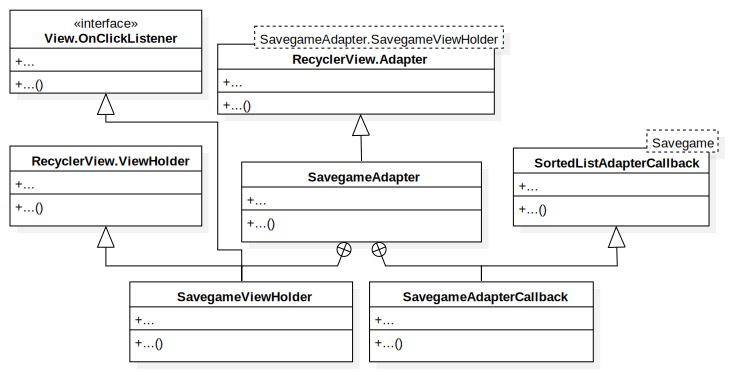
\includegraphics[width=1.0\textwidth]{resources/savegamestorage/SavegameAdapter}
	\caption{Spielstand SavegameAdapter}
\end{figure}

\subsection{Aufbau}
\subsectionauthor{\frank}

Wenn ein Spiel gespeichert oder geladen werden soll, geschieht dies durch einen
Aufruf der Instanz \code{SavegameStorage}. Um hier nicht mehrmals neuen Code,
welche alle Spiele gemeinsam haben, schreiben zu müssen, haben wir diese
Aufgabe an die Klasse \code{GameActivity} abgegeben. Da nun jedes Spiel von
\code{GameActivity} erben soll, müssen dadurch unter anderem zwei abstrakte
Methoden -- zum Speichern und Laden -- implementiert werden.
\code{onSaveGame(Bundle)} respektive \code{onLoadGame(Bundle)}. Diese Methoden
arbeiten jeweils mit einem \textbf{Bundle}, welchem die für einen
Speicherzustand nötigen Informationen übergeben beziehungsweise entnommen
werden können.

\begin{mdframed}[frametitle=Erklärung: Bundle]
Dies ist ein Objekt welches verschiedene Datentypen, wie zum Beispiel:
\emph{String, int} oder \emph{long}, mit \emph{String-Keys mapped} und hochperfomant
für \emph{Interprozesskommunikation} ist.
\end{mdframed}

 \unsure{Diesen Absatz eher in die Implementierung, oder?}
Das der Methode \code{onSaveGame} übergebene Bundle kann mit Methoden wie
\code{.putString} oder \code{.putStringArrayList} mit gefüttert werden.
Anschließend werden die gespeicherten Werte weiterverarbeitet und
abgespeichert. Das bedeutet, falls das Bundle unangetastet bleibt, kann
signalisiert werden, dass kein Speichern gewünscht ist, und so der Spielstand
nicht überschrieben wird. Dies ist sehr hilfreich, wenn ein Spiel gestartet,
der Zustand diesen aber nicht verändert wurde. So wird verhindert, dass die
Spielstandliste mit Startaufstellungen von Spielen überfüllt wird. Support für
das Löschen eines Spielstandes ist an dieser Stelle zum aktuellen Zeitpunkt
noch nicht vorhanden.

\let\thefootnote\relax\footnote{Ein Klassendiagramm der Spielstände, ist im Anhang zu finden.}
\chapter{Implementierung}

\section{Chess}
\sectionauthor{\oliver}

Schach ist eins der bekanntesten und gleichzeitig eins der anspruchsvollsten Spiele der Welt. Aufgrund der Komplexität
und benötigten Weitsichtigkeit schaffte es erst 1996 der Schachcomputer "Deep Blue" vom IBM den damalig amtierenden
Schachweltmeister Garro Kasparow zu besiegen. Heutzutage existieren viele Implementiereungen fähiger
Schachprogramme und KI`s. In diesem Projekt wurde wurde "Carballo" genommen.\unsure{Kommt das hier überhaut hin? Wenn ja, mehr?}

\subsection{Das Spielfeld}

Für das klassische karierte Spielfeld wurde die Klasse \code{CheckeredGameboardView} erstell,
welche wie der Name schon sag von der Androidklasse \code{View} erbt. Haputbestandteil ist ein
Zweidimensionales Array aus Androids\code{Rect}, welche die einzelnen Felder des Spielfelds darstellen.
Diese werden nach Aufruf von \code{onSizeChanged} der Größe des Displays angepasst und je nach
Einstellung um die Stärke des gewünschten Randes verschoben, sodass auf jedem Gerät ein identisches
Spielerlebnis erzegut werden kann. Um bei einem Touch auf die View zu ermitteln, auf welches der
Felder getippt wurde setzt die Methode \code{getSquareFromTouch(int x, int y)} die in \code{Rect}
mitgelieferte Funktion \code{contains(int x, int y)} ein und gibt die Array-Koordinaten des gesuchten
Kastens zurrück. Bei der Colorierung und Markierung der Felder bezieht sich die Klasse auf die in den
Einstellungen gespeicherten Werte.

\subsection{Der Chesswrapper}

In der Welt der Informatik sucht man den Begriff \emph{"Langlebig"} vergeblich, permanent werden
Module und Codeabschnitte verändert und ausgetauscht. Auch bei der Spielsammlung sind solche
Modifikationen vorgekommen und werden wohl in absehbarer Zeit wieder passieren. Aus diesem Grund
ist die Schachlogik nur über eine einzige Schnittstelle zugänglich, dem \code{ChessWrapper}. Dieser
umschließt alle benötigten Funktionen der verwendeten Schachbibliothek und erleichtert das Austauschen
der selbigen beachtlich. Neben grundlegenden Funktionen wie das ausgeben der aktuellen Figurenaufstellung
und das setzen von Schachzügen beinhaltet der Wrapper auch die Funktionen der künstlichen Intelligenz, welche
sich in der selben Bibliothek befindet. In zukünftigen Versionen werden diese Funktionen getrennt behandelt,
um allgemein geltenden Codemetriken gerecht zu werden.\unsure{Soll das so bleiben oder kommt das so rüber als ob wir das schlecht gemacht haben?}
\chapter{Evaluierung}

\section{Meinungen}

\begin{quote}
``Joa, ganz gut'' \\
``Die Karten kann man nicht so gut erkennen'' \\
``Aber sonst ist es so gut'' \\
``Die Navigation ist ziemlich einfach'' \\
``Die Hilfen [bei Schach] finde ich ganz gut'' \\
``Ich finde es gut, dass es mehrere Spiele zur Auswahl gibt''
\end{quote}
--- Lena, 14 Jahre, Schachanfängerin
\begin{quote}
``Die App ist einfach zu bedienen und macht Spaß'' \\
``Am Anfang ist die Startseite etwas leer'' 
\end{quote}
--- Tamara, 20 Jahre, 1. Semester Medieninformatik
\chapter{Ausblick}
\chapterauthor{\frank}

Trotz des sehr großen Erfolges unseres Programmierprojektes, gibt es immer noch
Sachen, die man vielleicht doch noch zu unserer Applikation hinzufügen möchte.
Oder vielleicht gibt es ja Sachen, die es aufgrund der relativ kurzen Zeit nicht
hinein geschafft werden. Ein paar dieser Dinge und Ideen werden im Folgenden
aufgelistet.

\section{Module}

Mit unserem Projekt lassen sich ziemlich einfach neue Spiele hinzufügen. Alles,
was man dafür tun muss ist, das Spiel in \code{games.xml} einzutragen und die
benötigten Klassen und Resourcendateien hinzuzufügen. Auch die Vererbung von der
Klasse \code{GameActivity} erleichtert die ganze Sache ungemein.\\ Doch ein
großer Nachteil bleibt: Um ein neues Spiel hinzufügen zu können braucht man
immer noch Einsicht und Zugriff auf den Quellcode der Applikation. Wie wäre es,
wenn man Spiele einfach von einem Repository herunterladen könnte, um sie der
App hinzuzufügen? Das Format hierfür würde einer API entsprechen, die ein Spiel
ansprechen kann. Man kann es sich ähnlich wie eine Spielemodifikation für
Minecraft oder Factorio -- wer es kennt -- vorstellen. Das Spiel wird als
ZIP-Datei in einen bestimmten Ordner eingefügt und kann dann beim Starten der
Applikation automatisch aus diesen Dateien geladen und dem Spielmenü hinzugefügt
werden. Die Struktur dieser Datei selbst würde aus einer Meta-Beschreibung des
Spiels und dem eigentlichen Spielinhalt bestehen. Diese Idee kann mit einem
zentralen Online-Repo und InApp-Downloadmöglichkeit verknüpft werden.

\section{Onlinespiele}

Aktuell ist man limitiert auf das Spielen an einem Gerät. Ob gegen den Computer
oder gegen den besten Freund gegenüber, beides ist möglich. Doch was ist, wenn
mal keinen Kumpel in der Nähe hat und die KI einem irgendwann langweilig wird?
Für den, der lieber im Keller sozial ist, wäre die Lösung: ein asynchroner
Onlinemodus. Hierfür werden die Spielstände zusammen mit Meta-Informationen, wie
etwa den beteiligten Spielern auf einem Server gespeichert. Anschließend kann
der gegnerische Spieler die entsprechenden Daten des Servers bei sich
herunterladen und den nächsten Zug ausführen. Das wäre ein ziemlich großes
Unterfangen, denn man braucht nicht nur die ganze Logik, die dahinter steckt,
sondern auch die Infrastruktur mit Datenbank und Wartungsarbeiten -- wie etwa
veraltete Spielstände zu löschen. Der Umfang hier wäre wieder in etwa so groß
wie die Dauer eines gesamten Programmierprojektes.
\input{sections/70_Fazit}
\input{sections/80_Tutorial}
\chapter{Anhang}

\section{Spielstände}
\sectionauthor{\leonard}

\begin{figure}[h]
	\centering
	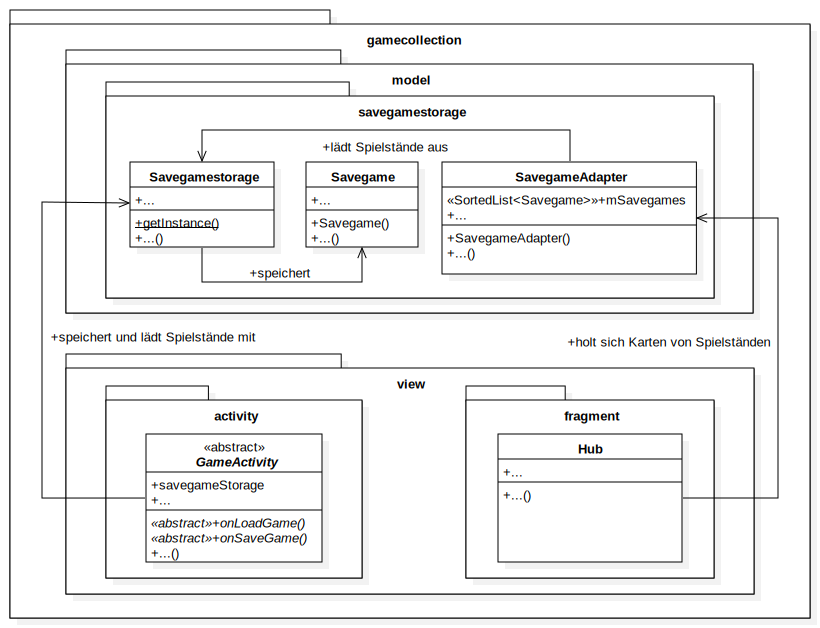
\includegraphics[width=1.0\textwidth]{resources/savegamestorage/Savegamestorage}
	\caption{Spielstand Architektur}
\end{figure}

\section{Schachavaluierung}

\begin{figure}[p]
\centering
\includegraphics[width=.3\textwidth]{resources/evaluierung/chess/screen}
\caption{Evaluierung: Der Schachbildschirm}
\label{fig:screen}
\end{figure}

\begin{figure}[p]
\centering
\includegraphics[width=.3\textwidth]{resources/evaluierung/chess/special}
\caption{Evaluierung: Aufstellung}
\label{fig:special}
\end{figure}

\begin{figure}[p]
\centering
\includegraphics[width=.3\textwidth]{resources/evaluierung/chess/checkmate}
\caption{Evaluierung: Schachmatt}
\label{fig:checkmate}
\end{figure}

\begin{figure}[h]
\centering
\includegraphics[width=.3\textwidth]{resources/evaluierung/chess/stalemate}
\caption{Evaluierung: Patt}
\label{fig:stalemate}
\end{figure}

\begin{figure}[h]
\centering
\includegraphics[width=.3\textwidth]{resources/evaluierung/chess/fifty_move}
\caption{Evaluierung: 50-Züge-Regel}
\label{fig:fifty_move}
\end{figure}

\begin{figure}[h]
\centering
\includegraphics[width=.3\textwidth]{resources/evaluierung/chess/castling_before}
\caption{Evaluierung: Rochade vorher}
\label{fig:castling_before}
\end{figure}

\begin{figure}[h]
\centering
\includegraphics[width=.3\textwidth]{resources/evaluierung/chess/castling_after}
\caption{Evaluierung: Rochade danach}
\label{fig:castling_after}
\end{figure}

\begin{figure}[h]
\centering
\includegraphics[width=.3\textwidth]{resources/evaluierung/chess/enpassant_before}
\caption{Evaluierung: En Passant vorher}
\label{fig:enpassant_before}
\end{figure}

\begin{figure}[h]
\centering
\includegraphics[width=.3\textwidth]{resources/evaluierung/chess/enpassant_after}
\caption{Evaluierung: En Passant danach}
\label{fig:enpassant_after}
\end{figure}

\begin{figure}[h]
\centering
\includegraphics[width=.3\textwidth]{resources/evaluierung/chess/promotion_dialog}
\caption{Evaluierung: Promotionsdialog}
\label{fig:promotion_dialog}
\end{figure}

\begin{figure}[h]
\centering
\includegraphics[width=.3\textwidth]{resources/evaluierung/chess/promotion_checkmate}
\caption{Evaluierung: Promotions-Schachmatt}
\label{fig:promotion_checkmate}
\end{figure}


\backmatter

%%%%%%%%%%%%%%%%%%%
%% create figure list
%%%%%%%%%%%%%%%%%%%


\listoffigures
\addcontentsline{toc}{chapter}{Verzeichnisse}			

%%%%%%%%%%%%%%%%%%%
%% create tables list
%%%%%%%%%%%%%%%%%%%
\listoftables

%%%%%%%%%%%%%%%%%%%
%% create listings list
%%%%%%%%%%%%%%%%%%%
\lstlistoflistings
\addcontentsline{toc}{chapter}{Listings}				


\printbibliography
\addcontentsline{toc}{chapter}{Literatur}				
\end{document}


